%***************************************
% Lab 05: Vending Machine
%***************************************
\chapter{Vending Machine}

\section{Purpose}

One of the important benefits of working with \textit{Logisim-evoluation} is being able to simulate real-world circuits before they are physically built. This lab simulates a vending machine that meets these requirements:

\begin{enumerate}
	\item The customer can input the following coins: 5-cent, 10-cent, 25-cent.
	\item When 75 cents is input, the machine will activate the dispenser and permit the customer to select a product.
	\item When at least 75 cents is input no more coins will be accepted.
	\item Change will be returned to the customer if more than 75 cents is deposited.
	\item A reset button will return the customer's money.
	\item When a product is dispensed, 75 cents will be added to the machine's ``Total Money Collected'' register.
	\item No product is dispensed if less than 75 cents is deposited.
	\item The current number of items available for each product is stored in a counter.
	\item When a service technician restocks the machine the item count for each product is set to 15, which is the maximum number of items that can be stocked.
	\item If the number of products available is zero for any one product the machine will light a ``sold out'' light and no action will be taken if that product is selected.
\end{enumerate}

This circuit uses only combinational logic and is an example of a reasonably complex system. 

\section{Procedure}

The starter circuit for this lab is almost complete, but three of the requirements have not been met.

\begin{itemize}
	\item Requirement three is that the coin input will stop once 75 cents is reached but this is not working so customers can continue depositing coins into the machine.
	\item When a product is dispensed, the coins deposited and change returned is not reset back to zero. This means that a customer could deposit 75 cents and then keep selecting products until the machine is empty.
	\item Requirement six is that the machine totals all of the money collected but that is not functional.
\end{itemize}

\subsection{Testing the Circuit}

To test the circuit:

\begin{enumerate}
	\item Ensure simulation is enabled at \textsc{Simulate -> Simulation Enabled}.
	\item Poke the \textit{Ena} input pin to enable the vending machine simulator.
	\item Notice that the \textit{SoldOut1}, \textit{SoldOut2}, and \textit{SoldOut3} LEDs are lit, indicating that those products are sold out.
	\item Restock products by poking the \textit{Restock1} and \textit{Restock2} buttons. For this test, do not poke \textit{Restock3} to keep that product empty. As a product is restocked the ``SoldOut'' LED for that product goes out.
	\item Poke the \textit{In5}, \textit{In10}, and \textit{In25} buttons to deposit coins. The total deposited is displayed and any amount over 75 cents is shown as change. Notice that the deposit circuit is not disabled after 75 cents is reached so customers can continue depositing coins.
	\item Once at least 75 cents is deposited, poke \textit{Vend1} to vend that product. The number of items available for that product decreases. Notice that once a product is dispensed the amount of money deposited is not reset and the machine can dispense additional products without additional money being deposited.
	\item Poke \textit{Vend3} and notice that nothing happens since that product is sold out.
	\item Poke \textit{Reset} to reset the amount of money deposited.
\end{enumerate}

\subsection{Subcircuit Descriptions}

This simulator contains five subcircuits in addition to the \lstinline[columns=fixed]|main| circuit and this section describes all of those components.

\subsubsection{main}

The \lstinline[columns=fixed]|main| circuit is the interface between a human customer and the simulator, as shown in Figure \ref{fig:05-01}. 

\begin{figure}[H]
	\centering
	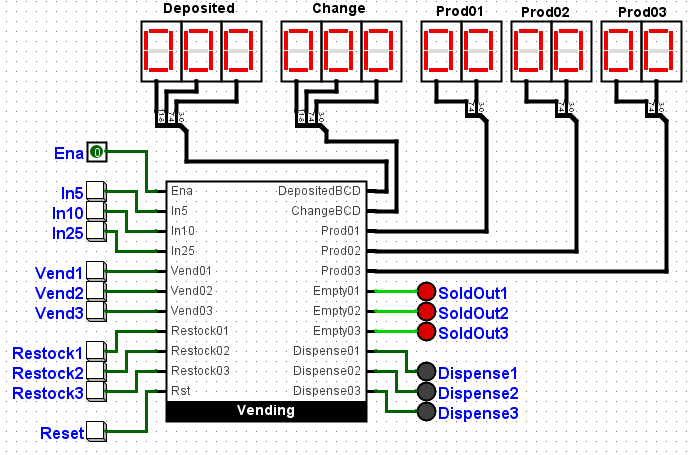
\includegraphics[width=\maxwidth{.95\linewidth}]{gfx/05-01}
	\caption{Vending Machine Main Circuit}
	\label{fig:05-01}
\end{figure}

The \lstinline[columns=fixed]|main| circuit includes the following components.

\begin{itemize}
	\item Numeric displays for the amount deposited, the change returned, and the number of items available for each of three products.
	\item An \textit{Ena} (\textit{Enable}) input so a technician can disable the machine for servicing.
	\item Buttons to simulate depositing coins, vending products, and restocking the machine.
	\item LEDs to indicate when products are sold out and dispensed.
\end{itemize}

\subsubsection{Activator}

The \lstinline[columns=fixed]|Activator| subcircuit receives a signal from the \lstinline[columns=fixed]|Bank| subcircuit that indicates how much money has been collected. The \lstinline[columns=fixed]|Activator| returns the \ac{BCD} Total and Change values and sets a signal to activate the \lstinline[columns=fixed]|Dispenser| subcircuit once 75 cents has been deposited. Figure \ref{fig:05-02} illustrates the \lstinline[columns=fixed]|Activator| subcircuit.

\begin{figure}[H]
	\centering
	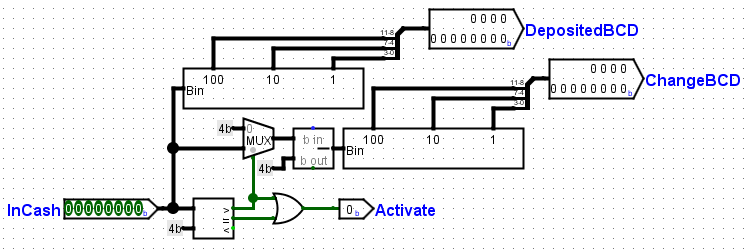
\includegraphics[width=\maxwidth{.95\linewidth}]{gfx/05-02}
	\caption{Activator Subcircuit}
	\label{fig:05-02}
\end{figure}

The \lstinline[columns=fixed]|Activator| subcircuit has only one input, \textit{InCash}. That input is connected to the \lstinline[columns=fixed]|Bank| subcircuit output and contains the total amount of cash deposited. That input is connected to a Bin2BCD (\textit{BFH mega functions} library) device and is then output as a \ac{BCD} number on the \textit{DepositedBCD} output pin.

The \textit{InCash} input is also sent to a comparator where the amount is compared to 75. If the amount in the bank is equal to or greater than 75 then the \lstinline[columns=fixed]|Activate| output goes high.

Finally, the \textit{InCash} input is sent to a mux that outputs 75 until the comparator indicates that more than 75 is in the bank, then the mux passes the \textit{InCash} amount to a subtractor where 75 is subtracted from it and the result sent to the \textit{ChangeBCD} output.

\subsubsection{Bank}

The \lstinline[columns=fixed]|Bank| subcircuit keeps a running total of the amount deposited and sends that total to the \lstinline[columns=fixed]|Activator| subcircuit. Figure \ref{fig:05-03} illustrates the \lstinline[columns=fixed]|Bank| subcircuit.

\begin{figure}[H]
	\centering
	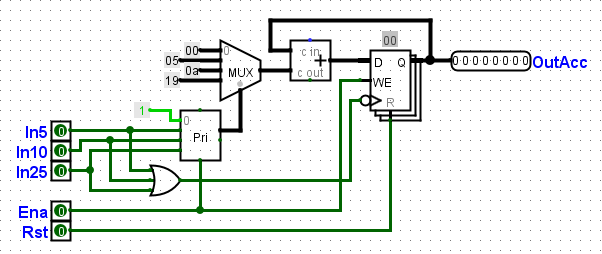
\includegraphics[width=\maxwidth{.95\linewidth}]{gfx/05-03}
	\caption{Bank Subcircuit}
	\label{fig:05-03}
\end{figure}

The \lstinline[columns=fixed]|Bank| subcircuit has five inputs. \textit{In5}, \textit{In10}, and \textit{In25} indicate the value of the coin dropped into the machine. When high, the \textit{Ena} input enables the \lstinline[columns=fixed]|Bank|. When high, the \textit{Rst} input resets the total to zero.

The \lstinline[columns=fixed]|Bank| subcircuit has only one output, \textit{OutAcc}, that makes the total cash accumulated available to the \lstinline[columns=fixed]|Activator| subcircuit.

For this description, imagine that a 5-cent coin is deposited. \textit{In5} goes high which changes the output of the priority encoder from zero to one. That output is sent to a mux control where the number five, on mux input one, is passed to an adder. The output of the adder is sent to a register where it is remembered. The output of the register is sent to the \textit{OutAcc} pin but is also looped back to the adder so each new coin is added to the previous total. Thus, the register keeps a running total of the money deposited.

The final logic function in this subcircuit is a three-input \texttt{OR} gate where each of the coin input pins are sent to the clock input of the register. As coins are dropped into the machine the register is clocked in order to capture each new deposit. It is important to note that \textit{the register is set to activate on a falling edge} in order to give the input signal enough time to propagate through the priority encoder, mux, and adder.

\subsubsection{Dispenser}

The \lstinline[columns=fixed]|Dispenser| subcircuit dispenses the three products available in the machine. Figure \ref{fig:05-04} illustrates the \lstinline[columns=fixed]|Dispenser| subcircuit.

\begin{figure}[H]
	\centering
	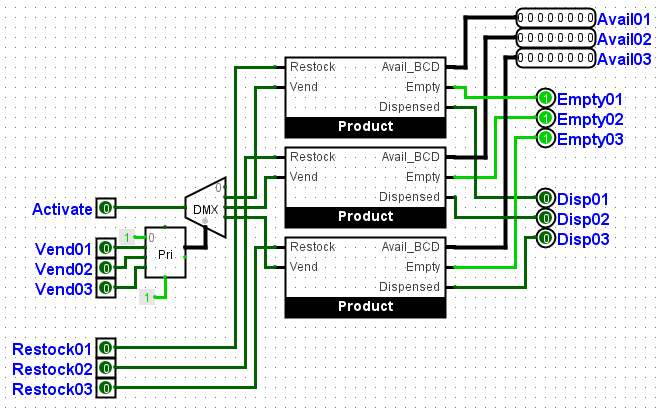
\includegraphics[width=\maxwidth{.95\linewidth}]{gfx/05-04}
	\caption{Dispenser Subcircuit}
	\label{fig:05-04}
\end{figure}

The Dispenser subcircuit has seven inputs and nine outputs.

Inputs:

\begin{itemize}
	\item \textbf{Activate}. A high input on this pin permits a product to be dispensed. This signal is generated in the \lstinline[columns=fixed]|Activator| subcircuit.
	\item \textbf{Vend}. These inputs cause one of three products to be dispensed.
	\item \textbf{Restock}. This resets the product count to 15, simulating a service technician restocking the machine.
\end{itemize}

Outputs:

\begin{itemize}
	\item \textbf{Avail}. This is an 8-bit number (not \ac{BCD}) that shows how many items each of the products have available for sale.
	\item \textbf{Empty}. This LED goes high when any product is sold out.
	\item \textbf{Disp}. This LED goes high when an item is dispensed.
\end{itemize}

Overall, this is a rather simple subcircuit. When one of the \textit{Vend} inputs goes high the priority encoder sends the number for that input to the demux control port. Thus, if a customer selects product one then the priority encoder transmits a one to the demux.

The demux will transmit the value present on the \textit{Activate} input to one of three \lstinline[columns=fixed]|Product| subcircuits. When \textit{Activate} is low then a zero is transmitted to the \lstinline[columns=fixed]|Product| subcircuit which effectively disables the dispenser function. However, if \textit{Activate} is high then a one is transmitted to one of the \lstinline[columns=fixed]|Product| subcircuits and that will cause a product to be dispensed.

\subsubsection{Product}

The \lstinline[columns=fixed]|Product| subcircuit keeps count of the number of items available for a product. There are two inputs and three outputs.

Inputs:

\begin{itemize}
	\item \textbf{Restock}. This resets the count of the item to 15. It is designed to simulate a service technician restocking the machine.
	\item \textbf{Vend}. When this goes high a single item is dispensed.
\end{itemize}

Outputs:

\begin{itemize}
	\item \textbf{AvailBCD}. This is a count, in \ac{BCD}, of the number of items available for sale.
	\item \textbf{Empty}. This goes high when there are no items available for sale.
	\item \textbf{Dispensed}. This goes high when an item is dispensed. It represents an item physically dropping out of the machine for the customer to retrieve.
\end{itemize}

\begin{figure}[H]
	\centering
	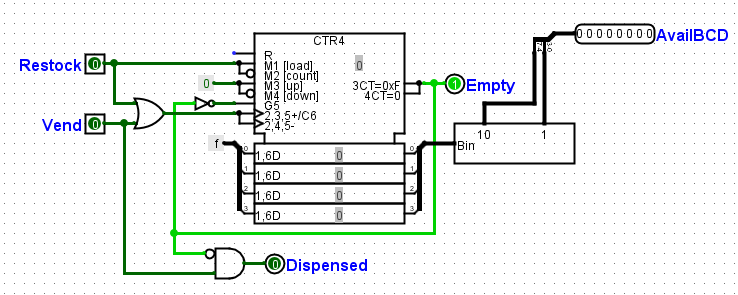
\includegraphics[width=\maxwidth{.95\linewidth}]{gfx/05-05}
	\caption{Product Subcircuit}
	\label{fig:05-05}
\end{figure}

This subcircuit is nothing more than a counter with a few controlling signals. The counter has a constant zero input on the \textit{M3} port. That sets the counter to decrement the count on each clock pulse.

The \textit{Restock} input is wired to the counter's reset port and a high input will reset the counter to 15. Note, the counter's properties are pre-set for a maximum count of 15.

The \textit{Vend} input is wired to the counter's clock port so when an item is sold the count will decrease. This input is also wired to the \textit{Dispensed} output to indicate that an item was sold.

The counter has two outputs. The \textit{3CT=0xF} output goes high when the count reaches zero (the item is sold out). That signal is used to disable the counter so no further sales are made. The second counter output is the count it contains and that is wired to a Bin2BCD (\textit{BFH mega functions} library) device. The output of that device is sent to the \textit{AvailBCD} port for other subcircuits to use.

\subsubsection{Vending}

The \lstinline[columns=fixed]|Vending| subcircuit consolidates the other subcircuits into an \ac{IC} that is used in the \lstinline[columns=fixed]|main| circuit. Figure \ref{fig:05-06} illustrates the \lstinline[columns=fixed]|Vending| subcircuit.

\begin{figure}[H]
	\centering
	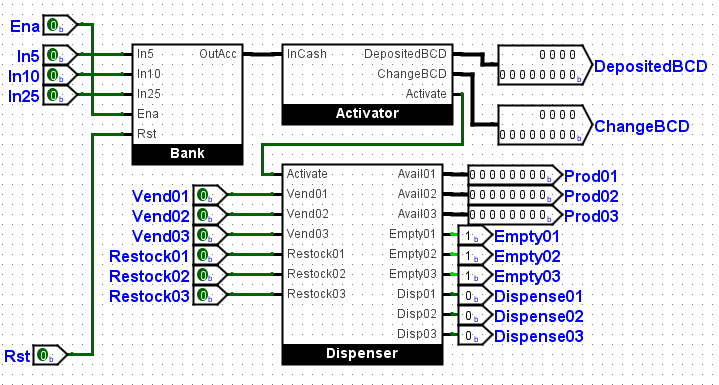
\includegraphics[width=\maxwidth{.95\linewidth}]{gfx/05-06}
	\caption{Vending Subcircuit}
	\label{fig:05-06}
\end{figure}

No further explanation is given for this subcircuit since it only wires the other subcircuits together and introduces no new logic.

\section{Challenge}

The Vending Machine simulator has three vital flaws that must be corrected.

\begin{itemize}
	\item Requirement three is that the coin input will stop once 75 cents is reached but this is not working so customers can continue depositing coins into the machine.
	\item When a product is dispensed, the coins deposited and change returned is not reset back to zero. This means that a customer could deposit 75 cents and then keep selecting products until the machine is empty.
	\item Requirement six is that the machine totals all of the money collected but that is not functional.
\end{itemize}


\section{Deliverable}

To receive a grade for this lab, correct all three flaws identified in the Challenge. Be sure the standard identifying information is at the top left of the \textit{main} circuit, similar to: 

\bigskip
% The minipage environment keeps the three lines together - no page break.
\begin{minipage}{\linewidth}
	\begin{verbatim}
	George Self
	Lab 05: Vending Machine
	February 16, 2018
	\end{verbatim}
\end{minipage}
\bigskip

Save the file with this name: \emph{\texttt{Lab05\_Vend}} and submit that file for grading.

